\documentclass[12pt,a4paper]{article}
\usepackage[utf8]{inputenc}
\usepackage{amsmath}
\usepackage{amsfonts}
\usepackage{amssymb}
\usepackage{graphicx}
\usepackage{geometry}
\usepackage{array}
\usepackage{tabularx}
\usepackage{booktabs}
\geometry{a4paper, margin=1in}
\usepackage{algorithm}
\usepackage{algpseudocode}
\usepackage{caption}
\usepackage[section]{placeins}
\usepackage{hyperref}
\hypersetup{hidelinks}
\captionsetup{font=small, skip=3pt}
\setlength{\textfloatsep}{10pt plus 2pt minus 2pt}
\setlength{\intextsep}{10pt plus 2pt minus 2pt}
\title{Particle Swarm Optimization (PSO): A Comprehensive Overview}
\author{}
\date{}
\begin{document}
\maketitle
\begin{abstract}
Particle Swarm Optimization (PSO) is a population-based stochastic optimization algorithm inspired by the social behavior of bird flocking and fish schooling. This report provides a comprehensive overview of the PSO algorithm, detailing its foundational concepts, mathematical implementation steps, real-world applications, an illustrative example, advanced variants, and related algorithms in the field of swarm intelligence.
\end{abstract}
\section{Introduction}
Introduced by James Kennedy and Russell Eberhart in 1995 \cite{kennedy1995}, Particle Swarm Optimization (PSO) is a metaheuristic optimization technique used to find the global optimum of a given objective function. Unlike traditional gradient-based methods, PSO does not require the optimization problem to be differentiable. Instead, it relies on a ``swarm'' of candidate solutions, known as particles, which explore the search space. 
Each particle moves through the multidimensional search space by adjusting its velocity and position based on two primary sources of information: its own personal experience (the best position it has found so far) and the collective experience of the swarm (the best position found by any particle in the group). This balance of exploration (searching new areas) and exploitation (refining known good areas) allows the swarm to converge toward an optimal solution efficiently.
\section{Steps to Implement PSO}
The standard PSO algorithm can be implemented through the following steps. The version below assumes a minimization objective; for maximization problems, the comparison signs in the personal-best and global-best updates should be reversed.
\begin{enumerate}
    \item \textbf{Initialization:} Initialize a swarm of $N$ particles. Assign each particle a random initial position $x_i(0)$ and a random initial velocity $v_i(0)$ within the boundaries of the $D$-dimensional search space.
    \item \textbf{Fitness Evaluation:} Evaluate the fitness of each particle by passing its current position $x_i(t)$ into the objective function $f(x)$.
    \item \textbf{Update Personal Best ($pBest$):} For each particle $i$, compare its current fitness with the fitness of its historical best position, $pBest_i$. If the current position is better, update $pBest_i = x_i(t)$.
    \item \textbf{Update Global Best ($gBest$):} Compare the $pBest$ of all particles to find the best overall position in the swarm. Update the global best position, $gBest$, if a better position is found.
    \item \textbf{Velocity Update:} Update the velocity of each particle for the next iteration using the following equation:
    \begin{equation}
        v_i(t+1) = w \cdot v_i(t) + c_1 \cdot r_1 \cdot (pBest_i - x_i(t)) + c_2 \cdot r_2 \cdot (gBest - x_i(t))
    \end{equation}
    Where:
    \begin{itemize}
        \item $w$ is the inertia weight (controls the impact of the previous velocity).
        \item $c_1$ and $c_2$ are cognitive and social acceleration coefficients.
        \item $r_1$ and $r_2$ are random vectors with components uniformly distributed in $[0, 1]$.
    \end{itemize}
    \textit{Optional:} A velocity clamping rule ($v_{\max}$) is often applied here to prevent particles from flying too far past the search space boundaries.
    \item \textbf{Position Update \& Boundary Handling:} Update the position of each particle:
    \begin{equation}
        x_i(t+1) = x_i(t) + v_i(t+1)
    \end{equation}
    If a particle moves outside the search bounds, boundary handling techniques (e.g., absorbing or reflecting walls) must be applied to bring it back into the valid space.
    \item \textbf{Termination:} Repeat steps 2 through 6 until a stopping criterion is met. Common stopping criteria include reaching a maximum number of iterations, observing only a small fitness improvement over a set number of iterations, or achieving a specific target error.
\end{enumerate}

\begin{algorithm}[H]
\caption*{PSO Pseudocode for Minimization}
\small
\begin{algorithmic}[1]
\State Initialize $N$ particles with random positions $x_i$ and velocities $v_i$
\State Evaluate fitness $f(x_i)$ for all particles
\State Set $pBest_i = x_i$ for all $i$
\State Set $gBest = \arg\min_{x_i} f(x_i)$
\While{stopping criterion is not met}
    \For{each particle $i = 1, \dots, N$}
        \State Update velocity: $v_i \gets w \cdot v_i + c_1 r_1 (pBest_i - x_i) + c_2 r_2 (gBest - x_i)$
        \State Update position: $x_i \gets x_i + v_i$
        \State Apply boundary handling if $x_i$ leaves the search space
        \If{$f(x_i) < f(pBest_i)$}
            \State $pBest_i \gets x_i$
        \EndIf
        \If{$f(pBest_i) < f(gBest)$}
            \State $gBest \gets pBest_i$
        \EndIf
    \EndFor
\EndWhile
\State \textbf{return} $gBest$
\end{algorithmic}
\end{algorithm}

\section{An Example Problem: Function Minimization}
To understand how PSO works in complex multimodal landscapes, consider the problem of finding the global minimum of the 2D Rastrigin function: 
\begin{equation*}
    f(x, y) = 20 + \left[x^2 - 10\cos(2\pi x)\right] + \left[y^2 - 10\cos(2\pi y)\right]
\end{equation*}
The Rastrigin function has dozens of deceptive local minima, but its true global minimum is at $(0,0)$ where $f(0,0) = 0$.

\medskip
\noindent
\begin{minipage}[t]{0.46\textwidth}
\textbf{Applying PSO:}
\begin{itemize}
    \item \textbf{Setup:} Initialize the swarm and trace Particle A at $(4,3)$ and Particle B at $(-2,1)$.
    \item \textbf{Initial fitness:} At integer coordinates, $\cos(2\pi n)=1$:
    \[
        f(A)=25,\qquad f(B)=5.
    \]
    Particle B is therefore the current $gBest$.
    \item \textbf{Movement:} Inertia carries Particle A forward, while the social term pulls it toward Particle B.
    \item \textbf{Convergence:} Repeated updates guide the swarm toward $(0,0)$, although exact convergence is not guaranteed.
\end{itemize}
\end{minipage}\hfill
\begin{minipage}[t]{0.50\textwidth}
    \centering
    \vspace{0pt}
    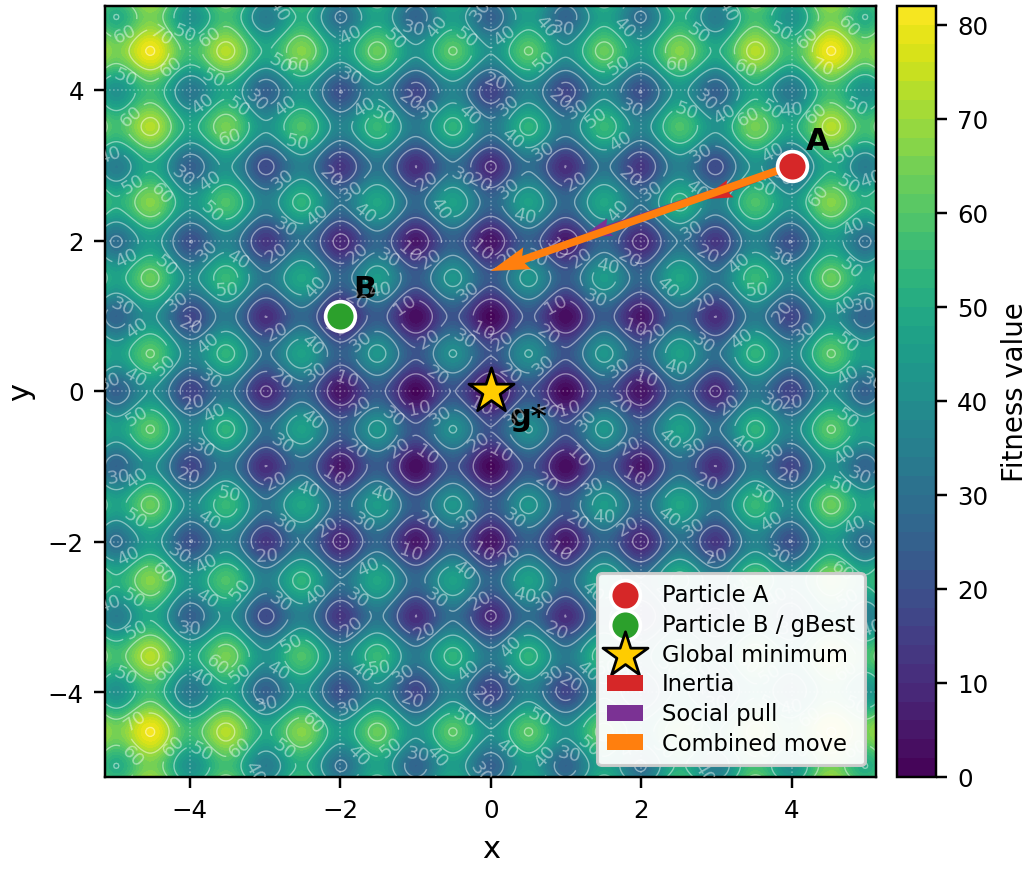
\includegraphics[width=\linewidth]{assets/pso_rastrigin_example.png}
    \captionof{figure}{One PSO movement step on the Rastrigin landscape. Particle A is influenced by its velocity and by the current global-best particle B.}
    \label{fig:pso_rastrigin}
\end{minipage}
\medskip

\begin{figure}[!htbp]
    \centering
    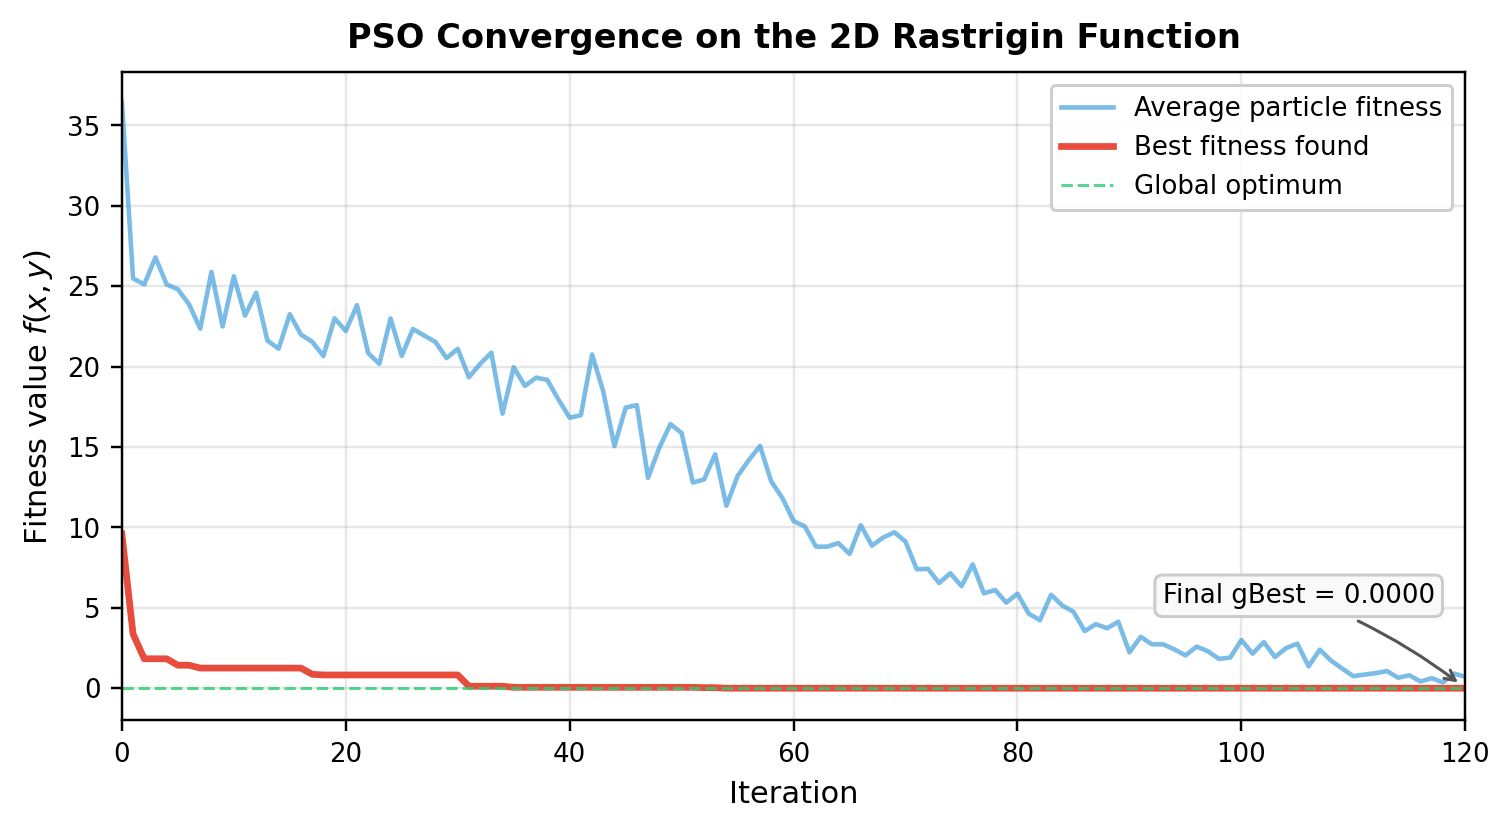
\includegraphics[width=0.74\textwidth]{assets/pso_rastrigin_convergence.png}
    \caption{Actual PSO convergence on the 2D Rastrigin example. The best fitness decreases over iterations as the swarm refines its search toward the known global minimum $f(0,0)=0$.}
    \label{fig:pso_rastrigin_convergence}
\end{figure}
\FloatBarrier

\section{Applications of PSO}
PSO has been widely applied across several domains because it is conceptually simple and adaptable to many optimization settings \cite{poli2007}:
\begin{itemize}
    \item \textbf{Machine Learning \& AI:} Optimizing weights and biases in Artificial Neural Networks (ANNs) and tuning hyperparameters for machine learning models.
    \item \textbf{Engineering Design:} Applied to complex, non-linear design tasks such as optimizing antenna array radiation patterns, reducing the weight of structures under stress constraints, and solving economic dispatch problems in power systems to minimize fuel costs.
    \item \textbf{Operations Research:} Used for logistical and scheduling challenges, including vehicle routing, resource allocation, and variants of the Traveling Salesman Problem. Because these are often discrete problems, they typically require modified or discrete PSO variants.
    \item \textbf{Robotics:} Often used for trajectory and path-planning optimization, helping autonomous robots and unmanned aerial vehicles (UAVs) search for smooth, collision-free routes.
    \item \textbf{Image Processing \& Healthcare:} Applied in computer vision tasks such as image segmentation and pattern recognition. In healthcare-related optimization, PSO can support medical image alignment, feature selection, and diagnostic model tuning.
\end{itemize}
\section{Upgraded Versions of PSO}
To overcome the limitations of the standard PSO, such as premature convergence to local optima, several upgraded variants have been developed:
\begin{itemize}
    \item \textbf{Adaptive PSO (APSO):} Dynamically adjusts parameters such as the inertia weight ($w$) and acceleration coefficients during the search process to balance exploration and exploitation \cite{zhan2009}.
    \item \textbf{Quantum-behaved PSO (QPSO):} Replaces the standard velocity update with a probabilistic particle-position model intended to improve global search \cite{sun2004}.
    \item \textbf{MOPSO:} Multi-Objective PSO uses Pareto dominance and an external archive to approximate trade-off solutions \cite{coello2004}.
    \item \textbf{Hybrid PSO:} Uses breeding and subpopulations to maintain diversity \cite{lovbjerg2001}.
\end{itemize}
\section{Related Algorithms: Comparisons with PSO}
PSO is part of a broader category of nature-inspired algorithms known as Swarm Intelligence. While sharing similarities, PSO differs significantly from its peers:

\begin{table}[htbp]
\centering
\small
\setlength{\tabcolsep}{6pt}
\renewcommand{\arraystretch}{1.18}
\begin{tabularx}{\textwidth}{@{}>{\raggedright\arraybackslash\bfseries}p{0.27\textwidth}>{\raggedright\arraybackslash}p{0.25\textwidth}>{\raggedright\arraybackslash}X@{}}
\toprule
Algorithm & \textbf{Inspiration} & \textbf{Comparison with PSO} \\ 
\midrule
Ant Colony Optimization (ACO) & Ant pheromone trails \cite{dorigo1996} & Primarily constructs solutions through pheromone-guided choices; standard PSO updates continuous position and velocity vectors. \\ 
Artificial Bee Colony (ABC) & Bee foraging roles \cite{karaboga2005} & Alternates employed-, onlooker-, and scout-bee phases; PSO updates every particle from personal and neighborhood best positions. \\ 
Genetic Algorithms (GA) & Selection, crossover, and mutation \cite{mitchell1998introduction} & Recombines selected solutions; PSO retains particle identities and moves them through the search space. \\ 
Differential Evolution (DE) & Scaled vector differences \cite{storn1997} & Generates trial vectors from population differences; PSO uses attraction toward remembered best positions. \\ 
\bottomrule
\end{tabularx}
\caption{Comparison of Swarm Intelligence and Evolutionary Algorithms}
\label{tab:comparisons}
\end{table}

\section{Limitations of PSO}
Although PSO is simple and effective, standard implementations have several limitations:
\begin{itemize}
    \item \textbf{Premature convergence:} Attraction to an early global-best position can reduce swarm diversity and trap particles around a local optimum \cite{poli2007}.
    \item \textbf{Parameter sensitivity:} The inertia weight and acceleration coefficients strongly affect stability, exploration, and convergence; unsuitable settings can produce oscillation, divergence, or slow progress \cite{clerc2002}.
    \item \textbf{Constraint and boundary handling:} The basic update equations do not enforce feasibility, so constrained problems require additional repair, penalty, or boundary-handling rules \cite{poli2007}.
    \item \textbf{No global-optimum guarantee:} Because PSO is stochastic, a run can return a near-optimal or local solution rather than the exact global optimum \cite{poli2007}.
\end{itemize}

\section{Conclusion}
PSO remains a widely used and flexible optimization algorithm. It is relatively easy to implement and can perform well on many continuous, nonlinear problems, but its effectiveness still depends on suitable parameter choices and problem-specific handling of constraints. Continued work on adaptive, multi-objective, quantum-behaved, and hybrid variants extends PSO to a broader range of optimization tasks.

\begin{thebibliography}{99}
\bibitem{kennedy1995} 
Kennedy, J. and Eberhart, R. (1995). 
\textit{Particle swarm optimization}. 
Proceedings of ICNN'95---International Conference on Neural Networks, vol. 4, pp. 1942--1948.
doi: \href{https://doi.org/10.1109/ICNN.1995.488968}{10.1109/ICNN.1995.488968}.

\bibitem{poli2007}
Poli, R., Kennedy, J., and Blackwell, T. (2007).
\textit{Particle swarm optimization}.
Swarm Intelligence, 1(1), 33--57.
doi: \href{https://doi.org/10.1007/s11721-007-0002-0}{10.1007/s11721-007-0002-0}.

\bibitem{zhan2009}
Zhan, Z.-H., Zhang, J., Li, Y., and Chung, H. S.-H. (2009).
\textit{Adaptive particle swarm optimization}.
IEEE Transactions on Systems, Man, and Cybernetics, Part B (Cybernetics), 39(6), 1362--1381.
doi: \href{https://doi.org/10.1109/TSMCB.2009.2015956}{10.1109/TSMCB.2009.2015956}.

\bibitem{sun2004}
Sun, J., Feng, B., and Xu, W. (2004).
\textit{Particle swarm optimization with particles having quantum behavior}.
Proceedings of the 2004 Congress on Evolutionary Computation, vol. 1, pp. 325--331.
doi: \href{https://doi.org/10.1109/CEC.2004.1330875}{10.1109/CEC.2004.1330875}.

\bibitem{coello2004}
Coello, C. A. C., Pulido, G. T., and Lechuga, M. S. (2004).
\textit{Handling multiple objectives with particle swarm optimization}.
IEEE Transactions on Evolutionary Computation, 8(3), 256--279.
doi: \href{https://doi.org/10.1109/TEVC.2004.826067}{10.1109/TEVC.2004.826067}.

\bibitem{lovbjerg2001}
L\o{}vbjerg, M., Rasmussen, T. K., and Krink, T. (2001).
\textit{Hybrid particle swarm optimiser with breeding and subpopulations}.
Proceedings of the Genetic and Evolutionary Computation Conference (GECCO 2001), pp. 469--476.

\bibitem{dorigo1996}
Dorigo, M., Maniezzo, V., and Colorni, A. (1996).
\textit{Ant system: optimization by a colony of cooperating agents}.
IEEE Transactions on Systems, Man, and Cybernetics, Part B (Cybernetics), 26(1), 29--41.
doi: \href{https://doi.org/10.1109/3477.484436}{10.1109/3477.484436}.

\bibitem{karaboga2005}
Karaboga, D. (2005).
\textit{An idea based on honey bee swarm for numerical optimization}.
Technical Report TR06, Erciyes University, Engineering Faculty, Computer Engineering Department.

\bibitem{mitchell1998introduction}
Mitchell, M. (1998).
\textit{An Introduction to Genetic Algorithms}.
MIT Press.

\bibitem{storn1997}
Storn, R. and Price, K. (1997).
\textit{Differential evolution---a simple and efficient heuristic for global optimization over continuous spaces}.
Journal of Global Optimization, 11(4), 341--359.
doi: \href{https://doi.org/10.1023/A:1008202821328}{10.1023/A:1008202821328}.

\bibitem{clerc2002}
Clerc, M. and Kennedy, J. (2002).
\textit{The particle swarm---explosion, stability, and convergence in a multidimensional complex space}.
IEEE Transactions on Evolutionary Computation, 6(1), 58--73.
doi: \href{https://doi.org/10.1109/4235.985692}{10.1109/4235.985692}.

\end{thebibliography}

\end{document}
